\documentclass[a4paper, 12pt]{article}
\usepackage{lmodern}
\usepackage{amssymb,amsmath}
\usepackage{ifxetex,ifluatex}
\usepackage{fixltx2e} % provides \textsubscript
\ifnum 0\ifxetex 1\fi\ifluatex 1\fi=0 % if pdftex
  \usepackage[T1]{fontenc}
  \usepackage[utf8]{inputenc}
\else % if luatex or xelatex
  \ifxetex
    \usepackage{mathspec}
  \else
    \usepackage{fontspec}
  \fi
  \defaultfontfeatures{Ligatures=TeX,Scale=MatchLowercase}
\fi
% use upquote if available, for straight quotes in verbatim environments
\IfFileExists{upquote.sty}{\usepackage{upquote}}{}
% use microtype if available
\IfFileExists{microtype.sty}{%
\usepackage{microtype}
\UseMicrotypeSet[protrusion]{basicmath} % disable protrusion for tt fonts
}{}
\usepackage[left=3cm,right=2cm,top=1.9cm,bottom=1.5cm,headheight=75pt,includeheadfoot]{geometry}
\usepackage{hyperref}
\PassOptionsToPackage{usenames,dvipsnames}{color} % color is loaded by hyperref
\hypersetup{unicode=true,
            pdftitle={Erros heteroscedástico-consistentes},
            pdfauthor={Luiz Fernando Palin Droubi; Norberto Hochheim; Willian Zonato},
            colorlinks=true,
            linkcolor=red,
            citecolor=green,
            urlcolor=magenta,
            breaklinks=true}
\urlstyle{same}  % don't use monospace font for urls
\usepackage{longtable,booktabs}
\usepackage{graphicx,grffile}
\makeatletter
\def\maxwidth{\ifdim\Gin@nat@width>\linewidth\linewidth\else\Gin@nat@width\fi}
\def\maxheight{\ifdim\Gin@nat@height>\textheight\textheight\else\Gin@nat@height\fi}
\makeatother
% Scale images if necessary, so that they will not overflow the page
% margins by default, and it is still possible to overwrite the defaults
% using explicit options in \includegraphics[width, height, ...]{}
\setkeys{Gin}{width=\maxwidth,height=\maxheight,keepaspectratio}
\IfFileExists{parskip.sty}{%
\usepackage{parskip}
}{% else
\setlength{\parindent}{0pt}
\setlength{\parskip}{6pt plus 2pt minus 1pt}
}
\setlength{\emergencystretch}{3em}  % prevent overfull lines
\providecommand{\tightlist}{%
  \setlength{\itemsep}{0pt}\setlength{\parskip}{0pt}}
\setcounter{secnumdepth}{5}
% Redefines (sub)paragraphs to behave more like sections
\ifx\paragraph\undefined\else
\let\oldparagraph\paragraph
\renewcommand{\paragraph}[1]{\oldparagraph{#1}\mbox{}}
\fi
\ifx\subparagraph\undefined\else
\let\oldsubparagraph\subparagraph
\renewcommand{\subparagraph}[1]{\oldsubparagraph{#1}\mbox{}}
\fi

%%% Use protect on footnotes to avoid problems with footnotes in titles
\let\rmarkdownfootnote\footnote%
\def\footnote{\protect\rmarkdownfootnote}

%%% Change title format to be more compact
\usepackage{titling}

% Create subtitle command for use in maketitle
\providecommand{\subtitle}[1]{
  \posttitle{
    \begin{center}\large#1\end{center}
    }
}

\setlength{\droptitle}{-2em}

  \title{Erros heteroscedástico-consistentes}
    \pretitle{\vspace{\droptitle}\centering\huge}
  \posttitle{\par}
  \subtitle{Teoria e simulações}
  \author{Luiz Fernando Palin Droubi\footnote{SPU/SC,
  \href{mailto:luiz.droubi@planejamento.gov.br}{\nolinkurl{luiz.droubi@planejamento.gov.br}}} \\ Norberto Hochheim\footnote{UFSC,
  \href{mailto:hochheim@gmail.com}{\nolinkurl{hochheim@gmail.com}}} \\ Willian Zonato\footnote{SPU/SC,
  \href{mailto:willian.zonato@planejamento.gov.br}{\nolinkurl{willian.zonato@planejamento.gov.br}}}}
    \preauthor{\centering\large\emph}
  \postauthor{\par}
      \predate{\centering\large\emph}
  \postdate{\par}
    \date{10/06/2019}

\usepackage[brazil]{babel}
\usepackage{graphicx}
\usepackage{float}
\usepackage{subfig}
\usepackage{caption}
\usepackage{lastpage}
%\usepackage{breqn}
\usepackage{booktabs}
\usepackage{longtable}
\usepackage{textcomp}
\usepackage{graphics}
\usepackage{lastpage}
\usepackage{lscape}
\setlength{\parindent}{1.25cm} % Default is 15pt.
\usepackage{indentfirst}
\usepackage{fontspec} % para Arial
\setmainfont{Arial}
\newcommand{\pkg}[1]{{\normalfont\fontseries{b}\selectfont #1}}
\let\proglang=\textsf
\let\code=\texttt
\usepackage{fancyhdr}
\renewcommand{\footrulewidth}{0.4pt}
\pagestyle{fancy}
\fancyhf{}
\fancyhead[CO,CE]{
  
\includegraphics[width=15mm, height = 11mm]{SPU.jpg}\\
  \textbf{MINISTÉRIO DA ECONOMIA}\\
    \textbf{SECRETARIA DE COORDENAÇÃO E GOVERNANÇA DO PATRIMÔNIO DA UNIÃO}\\
  SUPERINTENDÊNCIA DO PATRIMÔNIO DA UNIÃO EM SANTA CATARINA\\
  Praça XV de Novembro nº 336, Centro, Florianópolis/SC\\
  (48)3224-5399
}
\fancyfoot[CO, CE]{ARTIGO SUBMETIDO PARA A REVISTA XXX, JUNHO/2019
}
\fancyfoot[R]{\thepage~de~\pageref{LastPage}}

\begin{document}
\maketitle

\hypertarget{introducao}{%
\section{INTRODUÇÃO}\label{introducao}}

A homoscedasticidade é uma das hipóteses que devem ser necessariamente
verificadas na inferência clássica. A ausência da homoscedasticidade, ou
seja, a heteroscedasticidade, no entanto, não invalida completamente um
modelo de regressão linear, pois a heteroscedasticidade se relaciona
apenas aos erros do modelo, o que afeta o cômputo dos intervalos de
confiança das previsões e dos coeficientes do modelo, mas não invalida
os valores centrais dos mesmos, ou seja, mesmo que um modelo contenha
erros heteroscedásticos, este modelo pode ser utilizado para fazer
previsões, desde que não se esteja interessado nos seus intervalos de
confiança. Na Engenharia de Avaliações, contudo, frequentemente ou quase
sempre, existe interesse em avaliar o grau de precisão do modelo, ou
mesmo o grau de fundamentação de um laudo. Dado que estes enquadramentos
normativos são feitos com a utilização dos intervalos de confiança das
estimativas, ou com os p-valores dos testes de hipótese realizado pelos
regressores, a utilização de modelos com erros heteroscedásticos nesta
área torna-se complicada, o que não significa que isto seja impossível.
Infelizmente a NBR14.653-2 não aborda este assunto, mas acredita-se que,
mesmo assim, é possível se utilizar de modelos heteroscedásticos e ainda
estar de acordo com a norma. Demonstrar como isso pode ser feito é o
objetivo deste artigo.

\hypertarget{desenvolvimento-e-fundamentacao}{%
\section{DESENVOLVIMENTO E
FUNDAMENTAÇÃO}\label{desenvolvimento-e-fundamentacao}}

\hypertarget{a-hipotese-de-homoscedasticidade}{%
\subsection{A Hipótese de
homoscedasticidade}\label{a-hipotese-de-homoscedasticidade}}

Segundo Long (\protect\hyperlink{ref-Long}{2000}, p. 5), na regressão
linear, a variância do estimador MQO \(\hat{\beta}\) é:

\[\mathrm{var}(\hat{\beta})=(X'X)^{-1}X' \Omega X(X'X)^{-1}\]

A adoção da hipótese da homoscedasticidade na inferência clássica, em
conjunto com a hipótese da independência dos erros, pode ser resumida na
equação abaixo:

\[\Omega_{MQO}=\sigma^2I\] onde \(\sigma^2\) é a variância dos erros do
modelo, suposta constante, e \(I\) é a matriz identidade
\(n \text{x}n\), onde \(n\) é o número de dados do modelo. A matriz
\(\Omega\) assim obtida, pode-se demonstrar, simplifica demasiado o
cálculo da matriz de variância-covariância dos coeficientes de
estimação, da maneira a seguir:

\[\mathrm{var} (\hat{\beta})=\sigma^2(X'X)^{-1}\]

\hypertarget{deteccao-da-heteroscedasticidade}{%
\subsection{Detecção da
heteroscedasticidade}\label{deteccao-da-heteroscedasticidade}}

Diversos testes foram desenvolvidos visando a detecção da
heteroscedasticidade, dentro os quais citamos o teste de Goldfeld-Quandt
(\protect\hyperlink{ref-GQ}{1965}), o teste de Park
(\protect\hyperlink{ref-Park}{1966}), o teste de Glejser
(\protect\hyperlink{ref-glejser}{1969}), o teste de Breusch-Pagan
(\protect\hyperlink{ref-BP}{1979}) e o teste de White
(\protect\hyperlink{ref-white1980}{1980}).

Deve-se salientar que nenhum dos testes mencionados pode ser considerado
melhor do que o outro, porque, conforme será visto, cada um deles testa
uma hipótese em particular para a estrutura do erro. O teste de
Breusch-Pagan, por exemplo, assume que a estrutura da variância do termo
de erro seja linear, sendo muito eficiente para detectar este tipo de
heteroscedasticidade. Se, no entanto, se estiver lidando com uma
estrutura não-linear do termo de erro, este teste não será eficaz, sendo
o teste de White melhor para estes casos.

\hypertarget{teste-de-goldfeld-quandt}{%
\subsubsection{Teste de
Goldfeld-Quandt}\label{teste-de-goldfeld-quandt}}

O teste de Goldfeld-Quandt (\protect\hyperlink{ref-GQ}{1965}) é
aplicável a grandes amostras e consiste em omitir algumas amostras do
modelo e comparar a estrutura da variância do termo de erro em
diferentes subgrupos.

\hypertarget{teste-de-park}{%
\subsubsection{Teste de Park}\label{teste-de-park}}

O teste de Park (\protect\hyperlink{ref-Park}{1966}) assume que a
variância do termo de erro é proporcional a alguma potência da variável
independente (\(\sigma_{u_i}^2 = \sigma^2X_i^\beta e^v\)). Desta
maneira, o teste de Park consiste em estimar os resíduos da equação de
regressão e então fazer uso de uma regressão destes resíduos em relação
à variável dependente, da seguinte maneira:

\[ln(u_i^2) = ln(\sigma^2) + \beta ln(X_i) + v_i\] Se o coeficiente
\(\beta\) for significante, é indicativo da presença de
heteroscedasticidade.

\hypertarget{teste-de-glejser}{%
\subsubsection{Teste de Glejser}\label{teste-de-glejser}}

O teste de Glejser (\protect\hyperlink{ref-glejser}{1969}; \emph{apud}
NWAKUYA; NWABUEZE, \protect\hyperlink{ref-nigeria}{2018}) consiste em
testar se os valores absolutos dos resíduos (\(|\hat{u_i}|\)) da
regressão original tem correlação com alguma variável independente do
modelo (\(X_i\)), conforme formas abaixo:

\[|\hat{u_i}| = \beta_0 + \beta_1 X_i + v_i\]
\[|\hat{u_i}| = \beta_0 + \beta_1 \sqrt{X_i} + v_i\]
\[|\hat{u_i}| = \beta_0 + \beta_1 \frac{1}{X_i} + v_i\]
\[|\hat{u_i}| = \beta_0 + \beta_1 \frac{1}{\sqrt{X_i}} + v_i\]
\[|\hat{u_i}| = \sqrt{\beta_0 + \beta_1 X_i} + v_i\]
\[|\hat{u_i}| = \sqrt{\beta_0 + \beta_1 X_i^2} + v_i\]

\hypertarget{teste-de-breusch-pagan}{%
\subsubsection{Teste de Breusch-Pagan}\label{teste-de-breusch-pagan}}

O teste de Breusch-Pagan (\protect\hyperlink{ref-BP}{1979}) consiste em
assumir que a estrutura da variância do termo de erro seja linear em
função das variáveis independentes do modelo. Assim, o método consiste
em estimar a variância do erro à partir do quadrado dos resíduos da
regressão linear e efetuar então uma regressão auxiliar deste termo em
função dos regressores do mesmo modelo. Calcula-se o valor do
coeficiente de determinação deste modelo auxiliar e aplica-se o teste do
\(\chi^2\) para obter a sua significância. KOENKER
(\protect\hyperlink{ref-koenker1981}{1981}) propõe um ajuste ao teste
original, fazendo uso dos resíduos studantizados.

\hypertarget{teste-de-white}{%
\subsubsection{Teste de White}\label{teste-de-white}}

O teste de White (\protect\hyperlink{ref-white1980}{1980}) consiste numa
aplicação do teste de Breusch-Pagan, porém com a adição dos termos
quadráticos e de interação do modelo original. Obviamente, o teste de
White necessita de um número maios de graus de liberdade no modelo para
ter eficácio, haja vista que a regressão auxiliar necessitará de
diversos graus de liberdade.

\hypertarget{alternativas-para-contornar-a-heteroscedasticidade}{%
\subsection{Alternativas para contornar a
heteroscedasticidade}\label{alternativas-para-contornar-a-heteroscedasticidade}}

Ocorre que apenas raramente os dados do mundo real podem ser
considerados homoscedásticos e independentes, o que faz com que
procedimentos especiais tenham que ser tomados para a utilização do
estimador MQO. A tentativa de se contornar a heteroscedasticidade pode
ser feita de diversas formas, algumas mais trabalhosas, outras mais
complexas, outras causando maior distorção ao modelo.

\hypertarget{transformacao-da-variavel-dependente}{%
\subsection{Transformação da variável
dependente}\label{transformacao-da-variavel-dependente}}

Na Engenharia de Avaliações, a primeira e mais usual forma de se
contornar a heteroscedasticidade é através da aplicação de
transformações à variável dependente. No entanto, esta não é a única
alternativa e a transformação dos dados pode causar distorções
significativas, o que pode ser um problema, especialmente considerando o
problema da retransformação das variáveis transformadas.

Segundo MATLOFF (\protect\hyperlink{ref-matloff2017}{2017}), se
\(\varphi(x)\) é uma função convexa, então a desigualdade de Jensen se
exprime na seguinte desigualdade:

\[\varphi \left(\mathbb{E} [X]\right)\leq \mathbb{E} \left[\varphi (X)\right]\]

\hypertarget{outros-estimadores}{%
\subsection{Outros estimadores}\label{outros-estimadores}}

Outra forma de contornar a heteroscedasticidade é através da utilização
de outros estimadores, como o estimador dos mínimos quadrados
ponderados. Este método consiste na adoção de um vetor de pesos
conveninente escolhido e aplicado a cada uma das observações, de maneira
que se elimine a heteroscedasticidade do modelo. O inconveniente deste
método está na determinação do vetor de pesos a ser utilizado, o que não
é trivial.

\hypertarget{estimacao-heteroscedastico-consistente-da-matriz-de-variancia-covariancia}{%
\subsection{Estimação heteroscedástico-consistente da matriz de
variância-covariância}\label{estimacao-heteroscedastico-consistente-da-matriz-de-variancia-covariancia}}

Uma maneira mais interessante de se detectar a heteroscedasticidade é
através da estimação da matriz de variância-covariância dos coeficientes
heteroscedástico-consistente, desfazendo-se assim, da hipótese da
homoscedasticidade.

Existem diversas maneiras de se estimar a matriz
heteroscedástico-consistente, sendo que este método foi originalmente
concebido por White (\protect\hyperlink{ref-white1980}{1980};
\emph{apud} LONG; ERVIN, \protect\hyperlink{ref-Long}{2000}, p. 6), da
seguinte forma:

\[\text{HC0}=(X'X)^{-1}X' \hat{\Omega} X(X'X)^{-1} = (X'X)^{-1}X' diag[e_i^2] X(X'X)^{-1}\]
Onde \(diag[e_i^2]\) é a matriz diagonal em que os elementos da diagonal
são compostos pelo vetor do erros amostrais elevado ao quadrado.

Posteriormente diversas pequenas modificações foram propostas ao método,
como a correção dos resíduos pelos graus de liberdade (\(n/(n-k)\)) e
outras.

\hypertarget{estudo-de-caso}{%
\section{ESTUDO DE CASO}\label{estudo-de-caso}}

Para este estudo de caso foi utilizado software \proglang{R} 3.6.0. Os
funções utilizadas para a execução dos testes são do pacote \pkg{lmtest}
(ZEILEIS; HOTHORN, \protect\hyperlink{ref-lmtest}{2002}). Os gráficos
foram confeccionados com o auxílio do pacote \pkg{mosaic} (PRUIM et al.,
\protect\hyperlink{ref-mosaic}{2017}).

\hypertarget{exemplo-1}{%
\subsection{Exemplo 1}\label{exemplo-1}}

\hypertarget{criacao-dos-dados}{%
\subsubsection{Criação dos dados}\label{criacao-dos-dados}}

Neste primeiro exemplo foram gerados randomicamente para a variável
dependente (\(Y\)). Para a variável independente (\(X\)), foram criados
100 dados em sequência de 1 a 100. Para a varíavel dependente, com a
utilização da função \code{rnorm}, foram criados dados de distribuição
normal com média igual a média do vetor da variável independente
(\(\bar{Y} = \bar{X}\)) e desvio-padrão variável em função de \(X\), da
seguinte maneira:

\[\mathrm{desvio}(Y) = 0,4 \cdot X\] Ou seja, foi criada,
randômicamente, um tipo linear de heteroscedasticidade. Os gráfico dos
dados assim criados pode ser vistos na figura \ref{fig:hetero}.

\begin{figure}[H]

{\centering 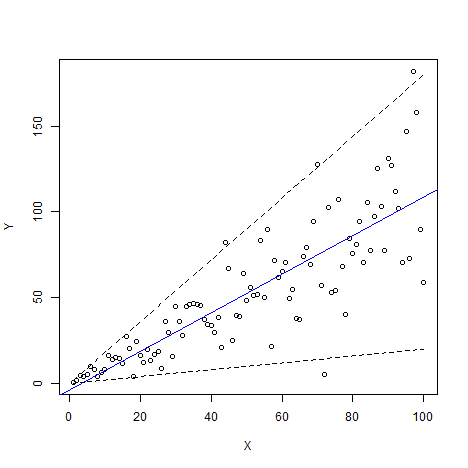
\includegraphics[width=0.6\linewidth]{images/hetero-1} 

}

\caption{Forma linear de heteroscedasticidade.}\label{fig:hetero}
\end{figure}

\hypertarget{testes}{%
\paragraph{Testes}\label{testes}}

Os resultados das estatísticas dos testes e suas significâncias estão
resumidos na tabela 1. Pode-se verificar que, para este caso, todos os
testes foram eficazes em não rejeitar a hipótese nula da
homoscedasticidade, ou seja, todos os testes detectaram a presença da
heteroscedasticidade.

\hypertarget{park}{%
\paragraph{Park}\label{park}}

Apesar da forma linear da heteroscedasticidade presente, como o valor da
estatística do teste t da variável \(\ln(X)\) resultou alto (5,48) e
significante (\(\text{p-valor} =\) 3.335e-07), conclui-se que não se
pode descartar a hipótese da heteroscedasticidade, ou seja, o teste de
Park funcionou, mesmo na presença de uma forma de heteroscedasticidade
diferente da pressuposta.

\hypertarget{glejser}{%
\paragraph{Glejser}\label{glejser}}

Foi utilizada a primeira forma (linear) do teste de Glejser. A
significância do teste foi de 3.55e-09. Conclui-se que o teste funciona.
Deve-se atentar, porém, que a forma de heteroscedasticidade, neste caso,
era previamente conhecida, o que possibilitou a aplicação da forma
``correta'' do teste, o que não ocorre na prática.

\hypertarget{breusch-pagan}{%
\paragraph{Breusch-Pagan}\label{breusch-pagan}}

A forma original do teste de BP foi aplicada, através da função
\code{bptest}:

O teste de BP, neste caso, não logrou a rejeição da hipótese nula, ou
seja, a da homoscedasticidade. Desta maneira, pode-se afirmar que o
teste funcionou a contento.

\hypertarget{breusch-pagan-studantizado-koenker}{%
\paragraph{Breusch-Pagan studantizado
(Koenker)}\label{breusch-pagan-studantizado-koenker}}

O mesmo ocorre para o teste de BP com a utilização dos resíduos
studantizados:

\hypertarget{goldfeld-quandt}{%
\paragraph{Goldfeld-Quandt}\label{goldfeld-quandt}}

O teste de GQ neste caso foi eficaz em detectar a modificação na
variância nas partições testadas.

\hypertarget{white}{%
\paragraph{White}\label{white}}

Por fim, o teste de White mostrou-se adequado para a detecção da forma
linear da heteroscedasticidade. No entanto, deve-se salientar, que para
isto foi inutilmente utilizado um grau de liberdade a mais do que o
teste de Breusch-Pagan, o que pode fazer a diferença no caso de pequenas
amostras.

\hypertarget{quadro-resumo}{%
\subsubsection{Quadro-Resumo}\label{quadro-resumo}}

\centerline{Tabela 1: Estatísticas e p-valores para os dados do Exemplo 1.}

\begin{longtable}[]{@{}lrr@{}}
\toprule
Teste & Estatística & Significância\tabularnewline
\midrule
\endhead
Park & 5,48 & 3.3e-07\tabularnewline
Glejser & 6,49 & 3.5e-09\tabularnewline
GQ & 15,95 & 2,5e-13\tabularnewline
BP & 40,28 & 2,2e-10\tabularnewline
Koenker & 18,86 & 1,4e-05\tabularnewline
White & 21,66 & 1,98e-05\tabularnewline
\bottomrule
\end{longtable}

\hypertarget{exemplo-2}{%
\subsection{Exemplo 2}\label{exemplo-2}}

\hypertarget{criacao-dos-dados-1}{%
\subsubsection{Criação dos dados}\label{criacao-dos-dados-1}}

Neste exemplo foram gerados randomicamente dados de distribuição normal
para a variável dependente (\(Y\)), com a utilização da função
\code{rnorm}, com média igual a média do vetor da variável independente
(\(\bar{Y} = \bar{X}\)) e desvio-padrão variável em função de \(X\), da
seguinte maneira:

\[\mathrm{desvio}(Y) = 0,001 \cdot X^2\]

Ou seja, foi criada, randômicamente, um tipo suavemente não-linear de
heteroscedasticidade. Os gráfico dos dados assim criados pode ser vistos
na figura \ref{fig:hetero2}.

\begin{figure}[H]

{\centering 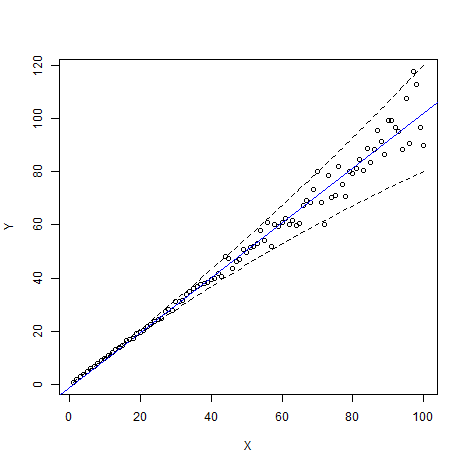
\includegraphics[width=0.6\linewidth]{images/hetero2-1} 

}

\caption{Forma não-linear de heteroscedasticidade.}\label{fig:hetero2}
\end{figure}

\hypertarget{testes-1}{%
\subsubsection{Testes}\label{testes-1}}

Os resultados das estatísticas dos testes e suas significâncias estão
resumidos na tabela 2. Pode-se verificar que, para este caso, todos os
testes foram eficazes em não rejeitar a hipótese nula da
homoscedasticidade, ou seja, todos os testes detectaram a presença da
heteroscedasticidade.

\hypertarget{park-1}{%
\paragraph{Park}\label{park-1}}

Apesar da forma linear da heteroscedasticidade presente, como o valor da
estatística do teste t da variável \(\ln(X)\) resultou alto (5,64) e
significante (\(\text{p-valor} =\) 1.652e-07), conclui-se que não se
pode descartar a hipótese da heteroscedasticidade, ou seja, o teste de
Park funcionou, mesmo na presença de uma forma de heteroscedasticidade
diferente da pressuposta.

\hypertarget{glejser-1}{%
\paragraph{Glejser}\label{glejser-1}}

Foi utilizada a primeira forma (linear) do teste de Glejser. A
significância do teste foi de 3.55e-09. Conclui-se que o teste funciona.
Deve-se atentar, porém, que a forma de heteroscedasticidade, neste caso,
era previamente conhecida, o que possibilitou a aplicação da forma
``correta'' do teste, o que não ocorre na prática.

\hypertarget{breusch-pagan-1}{%
\paragraph{Breusch-Pagan}\label{breusch-pagan-1}}

O teste de BP, apesar de assumir a forma linear de heteroscedasticidade,
logrou a rejeição da hipótese da homoscedasticidade. Isto ocorreu,
talvez, pela não-linearidade da heteroscedasticidade, neste caso, ser
singela.

\hypertarget{breusch-pagan-studantizado-koenker-1}{%
\paragraph{Breusch-Pagan studantizado
(Koenker)}\label{breusch-pagan-studantizado-koenker-1}}

O mesmo ocorre para ao teste de BP studantizado.

\hypertarget{goldfeld-quandt-1}{%
\paragraph{Goldfeld-Quandt}\label{goldfeld-quandt-1}}

O teste de Goldfeld-Quandt foi eficaz também neste caso, detectando a
presença da heteroscedasticidade.

\hypertarget{white-1}{%
\paragraph{White}\label{white-1}}

Por fim, o teste de White, concebido para encontrar as formas
não-lineares de heteroscedasticidade, também foi eficaz neste caso,
rejeitando a hipótese nula da homoscedasticidade.

\hypertarget{quadro-resumo-1}{%
\subsubsection{Quadro-Resumo}\label{quadro-resumo-1}}

\centerline{Tabela 2: Estatísticas e p-valores para os dados do Exemplo 2.}

\begin{longtable}[]{@{}lrr@{}}
\toprule
Teste & Estatística & Significância\tabularnewline
\midrule
\endhead
Park & 5,64 & 1.7e-07\tabularnewline
Glejser & 6,49 & 3.5e-09\tabularnewline
GQ & 220,9 & 5,4e-29\tabularnewline
BP & 71,84 & 2,3e-17\tabularnewline
Koenker & 20,96 & 4,68e-06\tabularnewline
White & 30,68 & 2,18e-07\tabularnewline
\bottomrule
\end{longtable}

\hypertarget{exemplo-3}{%
\subsection{Exemplo 3}\label{exemplo-3}}

\hypertarget{criacao-dos-dados-2}{%
\subsubsection{Criação dos dados}\label{criacao-dos-dados-2}}

Os dados foram criados da mesma maneira do exemplo anterior, porém com
uma nova função para a variância, da seguinte maneira:

\[\mathrm{desvio}(Y) = 0,5 \cdot (X-1)^2\]

Ou seja, foi criada, randômicamente, um tipo de heteroscedasticidade
não-linear mais drástico, onde a variância é menor no centro da amostra,
aumentando nas extremidades. Os gráfico dos dados assim criados pode ser
vistos na figura \ref{fig:hetero3}.

\begin{figure}[H]

{\centering 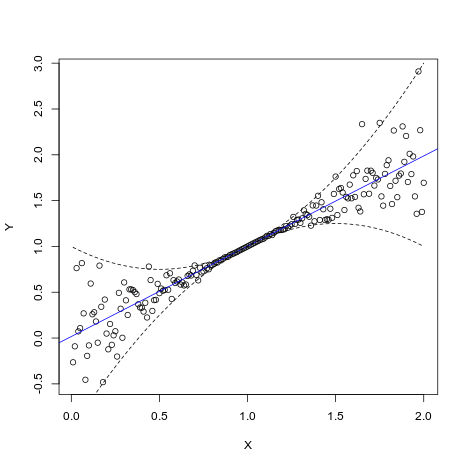
\includegraphics[width=0.6\linewidth]{images/hetero3-1} 

}

\caption{Forma drasticamente não-linear de heteroscedasticidade.}\label{fig:hetero3}
\end{figure}

\hypertarget{testes-2}{%
\subsubsection{Testes}\label{testes-2}}

\hypertarget{park-2}{%
\paragraph{Park}\label{park-2}}

Como o valor da estatística do teste t da variável \(\ln(X)\) resultou
alto (-3,09) e significante (\(\text{p-valor} =\) 0.002313), conclui-se
que não se pode descartar a hipótese da heteroscedasticidade.

\hypertarget{glejser-2}{%
\paragraph{Glejser}\label{glejser-2}}

Neste exemplo, o teste de Glejser detecta a heteroscedasticidade, mas
apenas na equação da forma quadrática, falhando em detectá-la na função
de teste linear.

Quando utilizada a forma quadrática do teste de Glejser. A significância
do teste foi de 0.0168.

\hypertarget{breusch-pagan-2}{%
\paragraph{Breusch-Pagan}\label{breusch-pagan-2}}

Na ocorrência da heteroscedasticidade não-linear extrema deste caso, o
teste de BP não logra a rejeição da hipótese nula, ou seja, a da
homoscedasticidade.

\hypertarget{breusch-pagan-studantizado-koenker-2}{%
\paragraph{Breusch-Pagan studantizado
(Koenker)}\label{breusch-pagan-studantizado-koenker-2}}

Também o teste de BP studantizado falha neste caso.

\hypertarget{goldfeld-quandt-2}{%
\paragraph{Goldfeld-Quandt}\label{goldfeld-quandt-2}}

Neste caso, o teste de Goldfeld=Quandt não logrou a rejeição da hipótese
nula, ou seja, a da homoscedasticidade, apesar de ser sabido que há
heteroscedasticidade no modelo. Ou seja, o teste falha em detectar a
heteroscedasticidade pela própria característica do mesmo, que divide em
a amostra em duas partições, excluindo-se uma fração dos dados centrais
(aqui 25\%) e compara suas variâncias. Como no presente caso a variância
muda igualmente em ambas as extremidades da amostra, o teste não a
detecta.

\hypertarget{white-2}{%
\paragraph{White}\label{white-2}}

Por fim, o teste de White mostrou-se adequado para a detecção da forma
de heteroscedasticidade drasticamente não-linear, como era de se
esperar.

\hypertarget{quadro-resumo-2}{%
\subsubsection{Quadro-Resumo}\label{quadro-resumo-2}}

\centerline{Tabela 3: Estatísticas e p-valores para os dados do Exemplo 3.}

\begin{longtable}[]{@{}lrr@{}}
\toprule
Teste & Estatística & Significância\tabularnewline
\midrule
\endhead
Park & -3,09 & 0.0023\tabularnewline
Glejser -- forma linear & 6,49 & 3.5e-09\tabularnewline
Glejser -- forma quadrática & 2,41 & 3.5e-09\tabularnewline
GQ & 1,071 & 0,39\tabularnewline
BP & 0,1466 & 0,7\tabularnewline
Koenker & 0,04362 & 0,835\tabularnewline
White & 47,36 & 5,21e-11\tabularnewline
\bottomrule
\end{longtable}

\hypertarget{conclusao}{%
\section{CONCLUSÃO}\label{conclusao}}

\hypertarget{referencias}{%
\section*{REFERÊNCIAS}\label{referencias}}
\addcontentsline{toc}{section}{REFERÊNCIAS}

\hypertarget{refs}{}
\leavevmode\hypertarget{ref-BP}{}%
BREUSCH, T. S.; PAGAN, A. R. A simple test for heteroscedasticity and
random coefficient variation. \textbf{Econometrica}, v. 47, n. 5, p.
1287--1294, 1979. {[}Wiley, Econometric Society{]}. Disponível em:
\textless{}\url{http://www.jstor.org/stable/1911963}\textgreater{}..

\leavevmode\hypertarget{ref-glejser}{}%
GLEJSER, H. A new test for heteroskedasticity. \textbf{Journal of the
American Statistical Association}, v. 64, n. 325, p. 316--323, 1969.
{[}American Statistical Association, Taylor \& Francis, Ltd.{]}.
Disponível em:
\textless{}\url{http://www.jstor.org/stable/2283741}\textgreater{}..

\leavevmode\hypertarget{ref-GQ}{}%
GOLDFELD, S. M.; QUANDT, R. E. Some tests for homoscedasticity.
\textbf{Journal of the American Statistical Association}, v. 60, n. 310,
p. 539--547, 1965. {[}American Statistical Association, Taylor \&
Francis, Ltd.{]}. Disponível em:
\textless{}\url{http://www.jstor.org/stable/2282689}\textgreater{}..

\leavevmode\hypertarget{ref-koenker1981}{}%
KOENKER, R. A note on studentizing a test for heteroscedasticity.
\textbf{Journal of Econometrics}, v. 17, n. 1, p. 107--112, 1981.
Disponível em:
\textless{}\url{http://www.sciencedirect.com/science/article/pii/0304407681900622}\textgreater{}..

\leavevmode\hypertarget{ref-Long}{}%
LONG, J. S.; ERVIN, L. H. Using heteroscedasticity consistent standard
errors in the linear regression model. \textbf{The American
Statistician}, v. 54, n. 3, p. 217--224, 2000. Taylor \& Francis.
Disponível em:
\textless{}\url{https://www.tandfonline.com/doi/abs/10.1080/00031305.2000.10474549}\textgreater{}..

\leavevmode\hypertarget{ref-matloff2017}{}%
MATLOFF, N. \textbf{Statistical regression and classification: From
linear models to machine learning}. Boca Raton, Florida: Chapman \&
Hall, 2017.

\leavevmode\hypertarget{ref-nigeria}{}%
NWAKUYA, M. T.; NWABUEZE, J. C. Application of Box-Cox transformation as
a corrective measure to heteroscedasticity using an economic data.
\textbf{American Journal of Mathematics and Statistics}, v. 8, n. 1, p.
8--12, 2018. Disponível em:
\textless{}\url{http://article.sapub.org/10.5923.j.ajms.20180801.02.html\#Ref}\textgreater{}..

\leavevmode\hypertarget{ref-Park}{}%
PARK, R. E. Estimation with heteroscedastic error terms.
\textbf{Econometrica}, v. 34, n. 4, p. 888--888, 1966. {[}Wiley,
Econometric Society{]}. Disponível em:
\textless{}\url{http://www.jstor.org/stable/1910108}\textgreater{}..

\leavevmode\hypertarget{ref-mosaic}{}%
PRUIM, R.; KAPLAN, D. T.; HORTON, N. J. The mosaic package: Helping
students to 'think with data' using r. \textbf{The R Journal}, v. 9, n.
1, p. 77--102, 2017. Disponível em:
\textless{}\url{https://journal.r-project.org/archive/2017/RJ-2017-024/index.html}\textgreater{}..

\leavevmode\hypertarget{ref-white1980}{}%
WHITE, H. A heteroskedasticity-consistent covariance matrix estimator
and a direct test for heteroskedasticity. \textbf{Econometrica}, v. 48,
n. 4, p. 817--38, 1980. Disponível em:
\textless{}\url{https://EconPapers.repec.org/RePEc:ecm:emetrp:v:48:y:1980:i:4:p:817-38}\textgreater{}..

\leavevmode\hypertarget{ref-lmtest}{}%
ZEILEIS, A.; HOTHORN, T. Diagnostic checking in regression
relationships. \textbf{R News}, v. 2, n. 3, p. 7--10, 2002. Disponível
em:
\textless{}\url{https://CRAN.R-project.org/doc/Rnews/}\textgreater{}..


\end{document}
